\section{Example trajectories and planning times}
\label{app:visualisations}
Stored seed-0 full-solver traces illustrate scenario types, including a
collision; they do not replace B4's repeated-run statistics. Squares mark
starts, stars goals, and crosses unfinished drones' returned positions.
Collision targets are not logged. Only the first sheet uses the demo's
9.5\,s allowance; later sheets use fixed-simulation experiments with relaxed
deadlines. The complete gallery covers all 76 evaluation configurations
and the supplied example, excluding development layouts.

\begin{figure}[H]
\centering
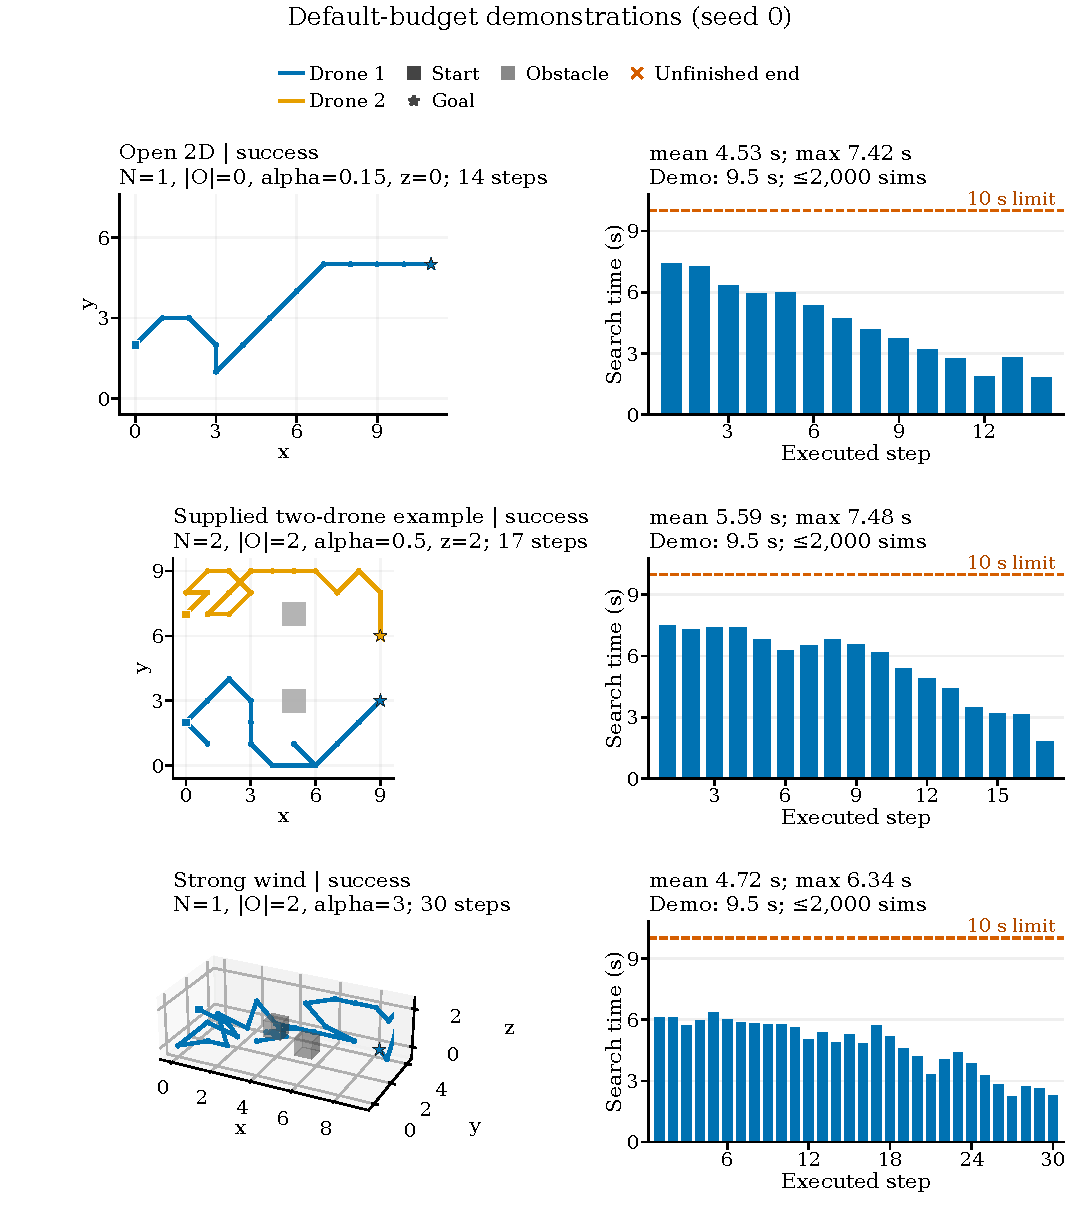
\includegraphics[width=\linewidth]{figures/scenario_examples_1.pdf}
\caption{Default-budget demonstrations: open navigation, the supplied
example, strong wind and four-drone 3D flight.}
\end{figure}

\clearpage
\begin{figure}[H]
\centering
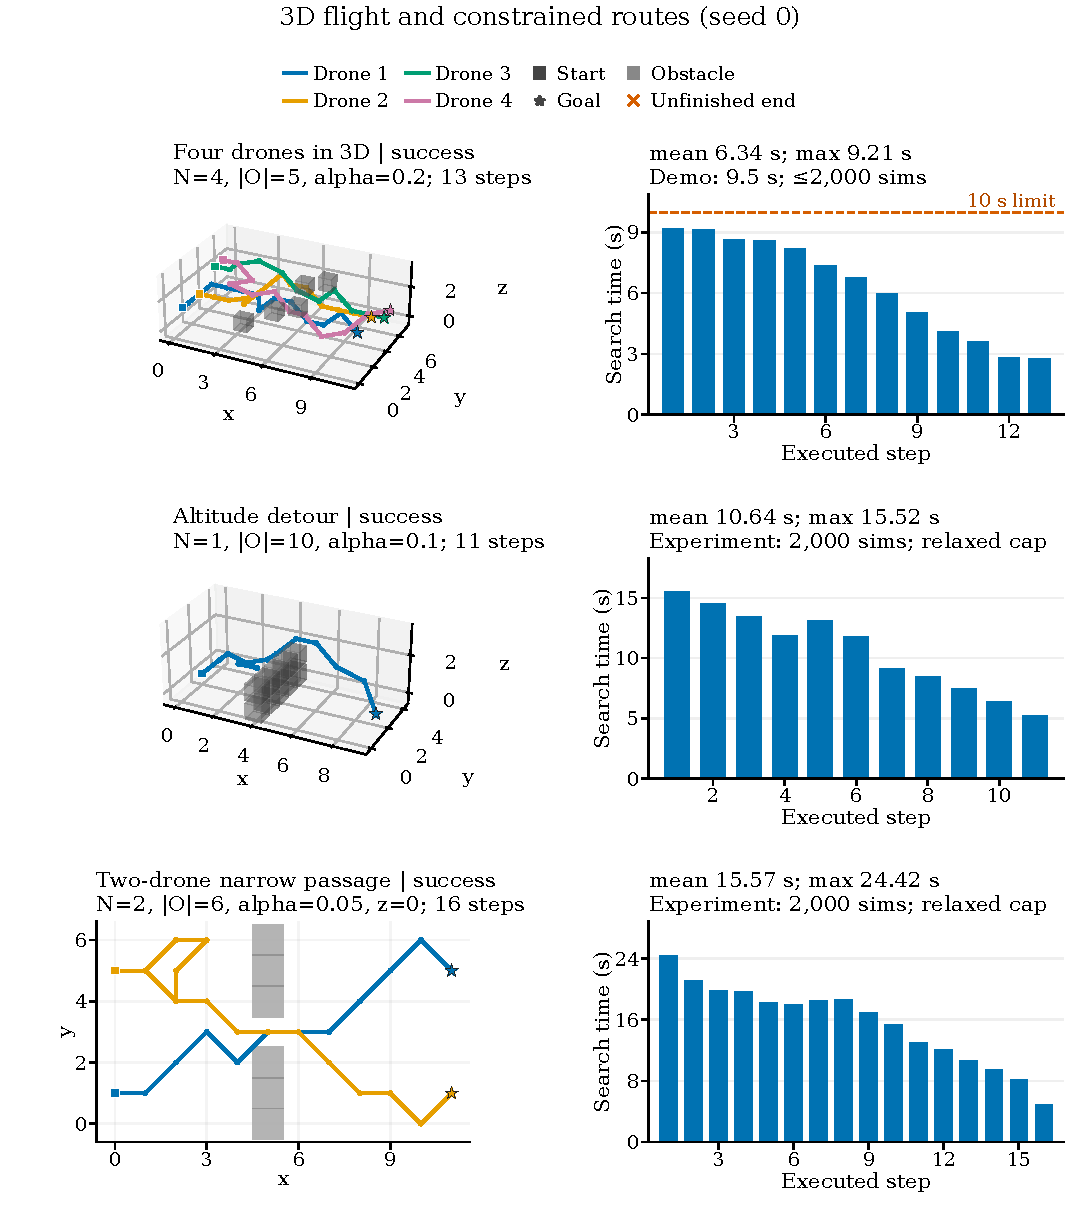
\includegraphics[width=\linewidth]{figures/scenario_examples_2.pdf}
\caption{Fixed-simulation examples: altitude detours, narrow passage,
clutter and a wall gap. The wall-gap layout has seven obstacles.}
\end{figure}

\clearpage
\begin{figure}[H]
\centering
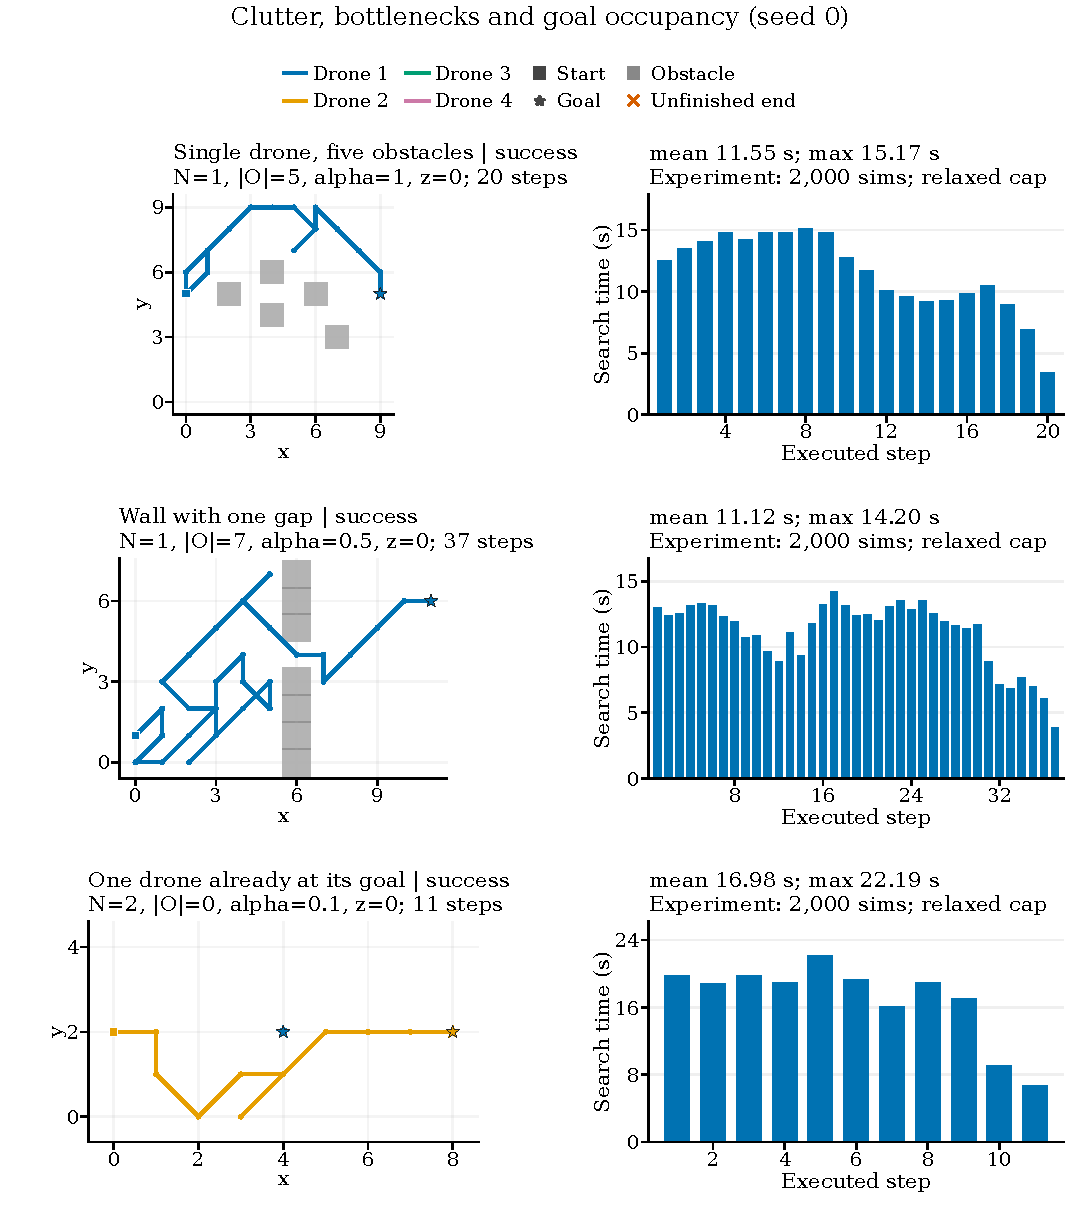
\includegraphics[width=\linewidth]{figures/scenario_examples_3.pdf}
\caption{Fixed-simulation examples: an occupied goal, separate altitude
layers, a shared corridor and a collision. The corridor has eight obstacles.
Timings on this and the preceding sheet are not demo deadline measurements.}
\end{figure}
